\section{Intro}

\begin{definition}{WEB-Architektur}
    \begin{itemize}
        \item Client-Server (Browser-Webserver)
        \item Interaktion: Request/Response
    \end{itemize}
    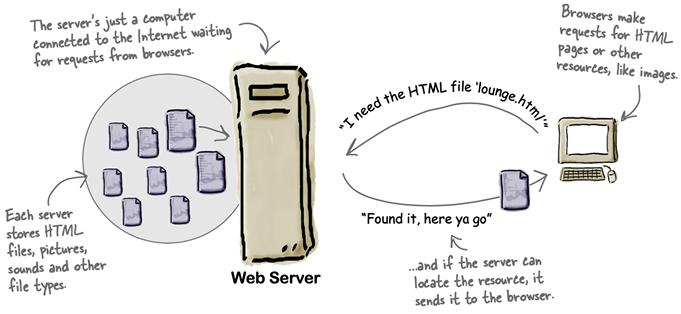
\includegraphics[width=1\linewidth]{images/web_architektur.png}
\end{definition}

\begin{concept}{Technologien}
    
    Client-Seitig
    \begin{itemize}
        \item Beschränkt auf das, was der Browser kann
        \item HTML + CSS + JavaScript + noch ein paar Sachen
        \item $\rightarrow$ Front-end Entwickler
    \end{itemize}

    Server-Seitig
    \begin{itemize}
        \item Praktisch unbeschränkt: Plattform, Programmiersprache, ...
        \item Erzeugt und gesendet wird das, was der Browser kann
        \item $\rightarrow$ Back-end Entwickler
    \end{itemize}
\end{concept}